% Line Atlas chapter draft.
% Suggested dependencies: amsmath, amssymb, siunitx, booktabs, tabularx,
% threeparttable, tikz, pgfplots, xcolor, hyperref.

\chapter{Line Formation and the Logic of Spectral Diagnostics}
\label{chap:line-formation-diagnostics}
\chaptermark{Line Formation and Diagnostics}

A spectrum contains many transitions but comparatively few independent pieces of
physical information.  Lines from a common ion share an abundance and ionization
fraction; multiplets share upper or lower states; every transition is filtered by the
same foreground dust and the same instrument.  The aim of diagnostic spectroscopy is
therefore not to attach one physical parameter to each line.  It is to identify line
combinations in which unwanted factors cancel and the desired dependence remains.
This chapter develops that logic for recombination lines, collisionally excited
lines, fine-structure transitions, resonance absorption, and molecules.  Standard
references include \citet{OsterbrockFerland2006}, \citet{DopitaSutherland2003},
\citet{Draine2011}, and \citet{Tielens2005}.

\section{Ionization balance is a rate problem}

The ionic abundance of an element is controlled by competing processes rather than
by a single ``formation temperature.''  In photoionized gas, a schematic balance
between stages $X^i$ and $X^{i+1}$ is
\begin{equation}
 n(X^i)\Gamma_i + n_en(X^i)C_i(T)
 =n_en(X^{i+1})\alpha_{i+1}(T)
  + n(X^{i+1})n_{\rm H^0}k_{\rm ce}(T),
 \label{eq:ionization-balance-general}
\end{equation}
where $\Gamma_i$ is a photoionization rate, $C_i$ a collisional ionization
coefficient, $\alpha_{i+1}$ the total radiative plus dielectronic recombination
coefficient, and $k_{\rm ce}$ represents charge exchange.  The photoionization rate
depends on the radiation field throughout the ionizing continuum,
\begin{equation}
 \Gamma_i=4\pi\int_{\nu_i}^{\infty}
 \frac{J_\nu}{h\nu}\sigma_i(\nu)\,\mathrm{d}\nu .
 \label{eq:photoionization-rate}
\end{equation}
An ionization threshold therefore does not specify the characteristic photon energy;
the product $J_\nu\sigma_i/\nu$ weights the actual photons doing the work.

The dimensionless ionization parameter is the number density of hydrogen-ionizing
photons relative to hydrogen atoms,
\begin{equation}
 U\equiv\frac{\Phi_{\rm H}}{n_{\rm H}c}
 =\frac{Q_{\rm H}}{4\pi r^2n_{\rm H}c}
 \label{eq:ionization-parameter}
\end{equation}
for an isotropic source emitting $Q_{\rm H}$ ionizing photons per second at distance
$r$.  A plane-parallel model often uses $U$ at its illuminated face; a spherical
nebula has a distribution of $U$.  Metal-line ratios can constrain $U$ only jointly
with spectral hardness, abundance pattern, pressure, and geometry.

In low-density, collisionally ionized equilibrium (CIE), ionization fractions are
primarily functions of temperature because both ionization and recombination rates
scale with $n_e$.  The familiar temperature at which an ion's CIE fraction peaks is
not a unique temperature of origin.  The same ion may exist in photoionized gas at a
much lower kinetic temperature, in a rapidly cooling nonequilibrium plasma, or at a
conductive or turbulent interface.  Thus O\,VI is evidence for highly ionized oxygen,
not by itself proof of gas at one particular temperature
\citep{GnatSternberg2007,TumlinsonPeeplesWerk2017}.

\subsection{Equilibrium timescales}

Equilibrium is plausible only if microscopic rates are fast compared with changes in
the gas.  A useful recombination timescale is
\begin{equation}
 t_{\rm rec}\simeq\frac{1}{\alpha(T)n_e}.
 \label{eq:recombination-timescale}
\end{equation}
At sufficiently low density, a radiation field or temperature can change faster than
ions recombine.  Cooling gas can then remain overionized relative to CIE, while gas
recently exposed to a source can remain underionized.  The diagnostic question is not
whether an equilibrium table exists, but whether $t_{\rm rec}$ and the ionization
timescale are short relative to the cooling, dynamical, and source-variability
timescales.

\section{Hydrogen and helium recombination spectra}

An ionizing photon absorbed by hydrogen creates a photoelectron.  Recombination and
cascade subsequently distribute photons among continua and lines.  In the standard
Case A idealization, every recombination line photon escapes.  In Case B, Lyman-series
photons are assumed optically thick and are converted through repeated absorption and
cascade, while most Balmer and longer-wavelength photons escape.  Neither case is a
universal property of an H\,II region; they are limiting transfer prescriptions
\citep{OsterbrockFerland2006}.

For an ionization-bounded nebula in steady state,
\begin{equation}
 Q_{\rm H,abs}=\int_V n_en_p\alpha_B(T)\,\mathrm{d}V,
 \label{eq:stromgren-balance}
\end{equation}
and a recombination-line luminosity is
\begin{equation}
 L_{ul}=h\nu_{ul}\frac{\alpha^{\rm eff}_{ul}(T)}{\alpha_B(T)}
 Q_{\rm H,abs}.
 \label{eq:recombination-luminosity-qh}
\end{equation}
This relation motivates H$\alpha$ and other recombination lines as star-formation
tracers.  It fails in predictable directions when ionizing photons escape, are
absorbed by dust, arise from an active nucleus or shocks, or when the assumed stellar
population does not represent the actual age and initial mass function
\citep{KennicuttEvans2012}.

\subsection{Balmer decrements and attenuation}

If the intrinsic ratio $R_{\rm int}=F({\rm H}\alpha)/F({\rm H}\beta)$ is known from
recombination theory, a foreground-screen color excess follows from
\begin{equation}
 E(B-V)=\frac{2.5}{k({\rm H}\beta)-k({\rm H}\alpha)}
 \log_{10}\!\left(\frac{R_{\rm obs}}{R_{\rm int}}\right),
 \label{eq:balmer-decrement-ebv}
\end{equation}
where $A_\lambda=k(\lambda)E(B-V)$.  This compact equation hides three model choices:
the intrinsic ratio depends weakly on temperature and density; the attenuation curve
must suit the source; and a mixed dust--emitter geometry is not a foreground screen.
Stellar Balmer absorption, flux-calibration slope, and differential aperture losses
can all bias $R_{\rm obs}$.  Infrared Paschen or Brackett lines extend the wavelength
lever arm and are less extinguished, but cross-instrument calibration can replace one
systematic with another \citep{Fitzpatrick1999}.

\subsection{Worked example: screen attenuation from
H\texorpdfstring{$\alpha$/H$\beta$}{-alpha/H-beta}}

Assume $R_{\rm obs}=4.0$, $R_{\rm int}=2.86$, and an adopted curve with
$k({\rm H}\beta)=3.61$ and $k({\rm H}\alpha)=2.53$.  Then
\begin{equation}
 E(B-V)=\frac{2.5}{1.08}\log_{10}(4.0/2.86)\simeq0.34~\mathrm{mag}.
\end{equation}
The attenuation correction to H$\alpha$ is
$10^{0.4k({\rm H}\alpha)E(B-V)}\simeq2.2$.  Reporting only the corrected luminosity
would conceal the dominant assumptions.  A reproducible measurement should state
the attenuation law, intrinsic decrement, stellar-continuum treatment, and whether
the correction refers to nebular or stellar reddening.

\section{Collisionally excited lines}

Forbidden and semiforbidden lines are not ``unlikely'' in the low-density universe.
Their small spontaneous rates allow metastable levels to radiate because the time
between particle collisions is long.  An excitation from $l$ to $u$ samples the
high-energy tail of the electron distribution through the exponential factor in the
rate coefficient.  A ratio of an auroral line from a high excitation energy to a
nebular line from a lower level can therefore be a sensitive electron thermometer.

For [O\,III], a commonly used conceptual ratio is
\begin{equation}
 R_{\rm OIII}=\frac{I(4959)+I(5007)}{I(4363)}.
 \label{eq:oiii-temperature-ratio}
\end{equation}
At densities below the relevant critical densities, $R_{\rm OIII}$ declines as
temperature rises because excitation of the auroral upper level becomes less
Boltzmann-suppressed.  At higher density, differential collisional de-excitation also
changes the ratio.  A five-level atom calculation, not a single analytic inversion,
is the normal inference tool.

Doublets such as [S\,II] $\lambda\lambda6716,6731$ or [O\,II]
$\lambda\lambda3726,3729$ compare levels close in energy but with different
collisional de-excitation rates.  Their ratios primarily constrain electron density,
but become insensitive at both low- and high-density limits.  Because a real aperture
contains a density distribution, the inferred ``density'' is an emissivity-weighted
effective value.

\begin{table}[tbp]
\centering
\caption{Diagnostic design patterns.  Entries describe the main sensitivity, not an
exclusive interpretation.  Atomic data and valid density ranges must accompany any
numerical calibration.}
\label{tab:diagnostic-design-patterns}
\begin{tabularx}{\textwidth}{@{}
 >{\raggedright\arraybackslash}p{0.22\textwidth}
 >{\raggedright\arraybackslash}p{0.28\textwidth}
 >{\raggedright\arraybackslash}X@{}}
\toprule
Pattern & Desired cancellation & Principal caveats \\
\midrule
Same-upper-level branching ratio & Population, abundance, and often temperature &
Differential extinction, blends, opacity, calibration; useful as an internal check \\
Auroral/nebular ratio of one ion & Ionic abundance and nearly all geometry &
Density dependence, recombination contribution, temperature gradients \\
Fine-structure doublet & Abundance and spectral hardness &
Low/high-density asymptotes, more than one collider \\
Adjacent ion stages of one element & Elemental abundance &
Ionization parameter entangled with spectral shape and geometry \\
Hydrogen recombination ratio & Emission measure and elemental abundance &
Transfer case, dust geometry, stellar absorption \\
Resonance-doublet apparent optical depth & Abundance scale and continuum &
Unresolved saturation, partial covering, scattered light \\
Isotopologue ratio & Much excitation physics if levels are matched &
Optical depth, isotope-selective chemistry, abundance-ratio variations \\
\bottomrule
\end{tabularx}
\end{table}

\section{Abundances: ionic measurements and ionization corrections}

An ionic abundance from an optically thin line ratio can be written schematically as
\begin{equation}
 \frac{n(X^i)}{n({\rm H}^+)}=
 \frac{I_\lambda(X^i)}{I({\rm H}\beta)}
 \frac{\epsilon_{{\rm H}\beta}(T,n_e)}
      {\epsilon_\lambda(X^i;T,n_e)}.
 \label{eq:ionic-abundance}
\end{equation}
The elemental abundance requires an ionization correction factor (ICF),
\begin{equation}
 \frac{X}{\mathrm{H}}=\mathrm{ICF}(X)
 \sum_{i\in\mathrm{observed}}\frac{X^i}{\mathrm{H}^+}.
 \label{eq:ionization-correction-factor}
\end{equation}
An ICF is a model statement about unobserved ions, not an observational constant.
It depends on the ionizing spectrum, geometry, and sometimes depletion into dust.

``Direct'' electron-temperature abundances are direct only in the limited sense that
a temperature-sensitive line is measured.  If temperature fluctuates spatially, the
auroral line weights hotter zones disproportionately because of its exponential
emissivity.  Recombination lines respond more weakly to temperature but are faint.
Strong-line metallicity calibrations trade weak-line sensitivity for dependence on a
model or empirical training set.  Different calibrations may differ systematically;
the calibration name and abundance scale are part of the result, not metadata that
can be omitted \citep{KewleyEllison2008,KewleyNichollsSutherland2019}.

\subsection{Ionization-source diagrams}

The Baldwin--Phillips--Terlevich family of diagrams compares a high-excitation line to
a Balmer line and a low-ionization line to another Balmer line
\citep{BaldwinPhillipsTerlevich1981}.  The closeness in wavelength of each ratio
reduces sensitivity to reddening and flux-calibration slope.  Star-forming sequences,
AGN, and shocks occupy different regions because their ionizing spectra and partially
ionized zones differ \citep{KewleyEtAl2001,KauffmannEtAl2003}.

Classification boundaries are not laws of nature.  Integrated spectra can mix H\,II
regions, diffuse ionized gas, shocks, and an AGN.  High-redshift abundance patterns,
pressures, and stellar spectra may shift the star-forming locus.  Spatially resolved
data are particularly vulnerable to low equivalent-width diffuse emission and to
point-spread-function mixing.  Diagnostic diagrams should be treated as projections
of a continuous mixture problem.

\begin{figure}[tbp]
\centering
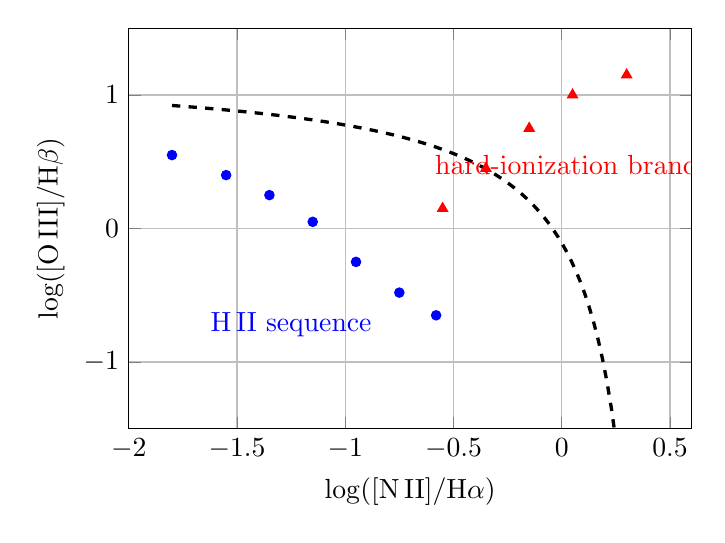
\begin{tikzpicture}
\begin{axis}[
 width=0.72\linewidth,height=0.55\linewidth,
 xlabel={$\log([\mathrm{N\,II}]/\mathrm{H}\alpha)$},
 ylabel={$\log([\mathrm{O\,III}]/\mathrm{H}\beta)$},
 xmin=-2.0,xmax=0.6,ymin=-1.5,ymax=1.5,
 grid=major,
]
 \addplot[only marks,mark=*,mark size=1.7pt,blue]
 coordinates {(-1.8,0.55) (-1.55,0.40) (-1.35,0.25) (-1.15,0.05)
 (-0.95,-0.25) (-0.75,-0.48) (-0.58,-0.65)};
 \addplot[only marks,mark=triangle*,mark size=2.1pt,red]
 coordinates {(-0.55,0.15) (-0.35,0.45) (-0.15,0.75) (0.05,1.0)
 (0.30,1.15)};
 \addplot[very thick,dashed,domain=-1.8:0.25,samples=100]
 {0.61/(x-0.47)+1.19};
 \node[blue] at (axis cs:-1.25,-0.72) {H\,II sequence};
 \node[red] at (axis cs:0.05,0.48) {hard-ionization branch};
\end{axis}
\end{tikzpicture}
\caption{Original PGFPlots concept for an emission-line diagnostic plane.  The
points are synthetic and the dashed curve is illustrative; the production caption
must identify any adopted empirical or theoretical boundary and its domain of
validity.}
\label{fig:diagnostic-plane-concept}
\end{figure}

\section{Fine-structure lines and infrared diagnostics}

Fine-structure transitions connect closely spaced levels within a ground electronic
term.  Their excitation energies correspond to tens to thousands of kelvin, making
them bright coolants of gas too cool to radiate optical collisionally excited lines.
Important examples include [C\,II] $158\,\mu$m, [O\,I] $63$ and $145\,\mu$m,
[O\,III] $52$ and $88\,\mu$m, [N\,II] $122$ and $205\,\mu$m, and [Ne\,II]
$12.8\,\mu$m.  Dust extinction is greatly reduced in the infrared, though dust
continuum opacity may still matter in compact, high-column sources.

Several colliders can excite the same line.  For [C\,II], electrons, H, and
H$_2$ have different rate coefficients and dominate in different phases.  An
observed [C\,II] luminosity can combine ionized gas, atomic photodissociation layers,
and CO-faint molecular envelopes.  [N\,II], which requires ionized gas, can help
estimate the ionized contribution if abundance and density are constrained.  A line
frequently used as a star-formation proxy is therefore not emitted by a single
``star-forming phase.''

The luminosity of a two-level fine-structure line per ion approaches a maximum in the
thermalized, optically thin limit.  Consequently line luminosity gives a strict
minimum mass of the emitting ion only after adopting temperature, collider density,
and upper-level fraction.  Optical depth and subcritical excitation increase the
required mass.

\section{Molecular rotational and vibrational lines}

For a linear rigid rotor with rotational constant $B$, idealized level energies are
\begin{equation}
 E_J=hBJ(J+1),\qquad g_J=2J+1,
 \label{eq:rigid-rotor}
\end{equation}
and allowed electric-dipole rotational transitions have $\Delta J=\pm1$ when the
molecule has a permanent dipole moment.  CO has low-lying transitions that are easy
to excite in cold molecular gas.  H$_2$ has no permanent dipole; its quadrupole
rotational lines require warmer material, so cold H$_2$ is usually inferred through
CO, dust, gamma rays, or absorption rather than direct emission.

If lines are optically thin, share one excitation temperature, and beam filling is
known, a rotational diagram uses
\begin{equation}
 \ln\!\left(\frac{N_u}{g_u}\right)
 =\ln\!\left(\frac{N_{\rm tot}}{Q(T_{\rm ex})}\right)
 -\frac{E_u}{kT_{\rm ex}}.
 \label{eq:rotational-diagram}
\end{equation}
The inverse slope is $-T_{\rm ex}$ and the intercept encodes total column through the
partition function $Q$.  Curvature can indicate multiple temperatures, non-LTE
populations, opacity, or inconsistent emitting areas.  A straight line does not prove
LTE; limited dynamic range can hide departures.

For unresolved sources, brightness-temperature line luminosity is often denoted
$L'$ in units of $\mathrm{K\,km\,s^{-1}\,pc^2}$.  Molecular mass is then
\begin{equation}
 M_{\rm mol}=\alpha_{\rm CO}L'_{\rm CO(1-0)},
 \label{eq:alpha-co}
\end{equation}
where the inclusion of helium must be stated.  The conversion factor varies with
metallicity, shielding, surface density, temperature, and dynamics; a Milky-Way disk
value should not be applied automatically to low-metallicity dwarfs or compact
starbursts \citep{BolattoWolfireLeroy2013}.

\subsection{Worked example: a two-line excitation temperature}

Suppose optically thin measurements yield upper-level columns $N_1$ and $N_2$ for
energies $E_1<E_2$.  Equation~\eqref{eq:rotational-diagram} gives
\begin{equation}
 T_{\rm ex}=\frac{E_2-E_1}{k}
 \left[\ln\!\left(\frac{N_1g_2}{N_2g_1}\right)\right]^{-1}.
 \label{eq:two-line-tex}
\end{equation}
Let $(E_2-E_1)/k=11.1$~K and
$N_1g_2/(N_2g_1)=2.0$.  Then $T_{\rm ex}=16.0$~K.  This is an excitation
temperature between two states, not necessarily the kinetic temperature.  If the
density is subcritical, radiative trapping or the cosmic microwave background can
set $T_{\rm ex}$.  At redshift $z$, the background temperature
$T_{\rm CMB}=2.725(1+z)$~K both excites the molecule and reduces observed contrast.

\section{Absorption-line column densities}

Normalized absorption directly measures apparent optical depth,
\begin{equation}
 \tau_a(v)=\ln\!\left[\frac{F_c(v)}{F(v)}\right],
 \label{eq:apparent-optical-depth}
\end{equation}
and the apparent column-density profile is
\begin{equation}
 N_a(v)=\frac{m_ec}{\pi e^2}
 \frac{\tau_a(v)}{f\lambda_0}.
 \label{eq:aod-column}
\end{equation}
In practical units,
\begin{equation}
 N_a(v)=3.768\times10^{14}
 \frac{\tau_a(v)}{f(\lambda_0/\text{\AA})}
 \quad \mathrm{cm^{-2}\,(km\,s^{-1})^{-1}}.
 \label{eq:aod-practical}
\end{equation}
Integrating over velocity yields an apparent ionic column.  Agreement between
$N_a(v)$ profiles for two transitions of the same ion with different $f\lambda$
supports adequate resolution.  A smaller apparent column in the stronger line flags
unresolved saturation \citep{SavageSembach1991,FoxSavageWakker2005}.

Partial covering changes the residual intensity to
\begin{equation}
 \frac{F(v)}{F_c}=1-C_f(v)+C_f(v)e^{-\tau(v)}.
 \label{eq:partial-covering}
\end{equation}
A saturated line can therefore have a nonzero core.  Scattered light, unrelated
continuum components, and instrumental background can produce the same symptom.
Doublet fitting may constrain $C_f$ and $\tau$, but only within the chosen geometry.

\section{Masers, inversions, and negative opacity}

If $n_u/g_u>n_l/g_l$, the stimulated-emission term exceeds true absorption and
$\alpha_\nu<0$.  Equation~\eqref{eq:homogeneous-slab} then describes exponential
amplification rather than attenuation.  Astrophysical masers require a pump that
creates the inversion, a velocity-coherent path, and a seed radiation field.
Unsaturated maser intensity grows approximately exponentially with path length;
saturation couples the radiation back to the level populations and limits growth.
Narrowness, high brightness temperature, variability, and polarization can reveal
masing, but isotropic luminosity is misleading because the emission may be strongly
beamed.

\section{A diagnostic is a model comparison}

Every line ratio can be written abstractly as a forward model
\begin{equation}
 \boldsymbol{F}_{\rm pred}=
 \mathcal{M}(T,n,\boldsymbol{Z},U,J_\nu,\boldsymbol{v},\mathcal{G},
 \boldsymbol{a}),
 \label{eq:diagnostic-forward-model}
\end{equation}
where $\mathcal{G}$ denotes geometry and $\boldsymbol{a}$ atomic or molecular data.
Inference asks which parameter combinations are consistent with measured fluxes and
their covariance.  A sound atlas therefore records for each diagnostic:
\begin{enumerate}
 \item the transitions and adopted atomic data;
 \item the dominant production and destruction mechanisms;
 \item the density, temperature, abundance, and ionization ranges over which the
 calibration was constructed;
 \item assumptions about equilibrium, opacity, geometry, and radiation field;
 \item known degeneracies and at least one independent cross-check;
 \item whether limits, nondetections, and calibration covariance were included.
\end{enumerate}
The value of a line lies not in a single canonical interpretation, but in knowing
precisely which physical alternatives it can distinguish.
